\documentclass[onecolumn]{article}
\usepackage{graphicx}

\begin{document}

\title{What is the largest triangle that fits in a square?}

\author{Arjen Markus}

\maketitle

\subsection*{Introduction}
While considering the smallest circle that encloses a set of points, I also wondered about
the problem of finding the smallest rectangle around such a set. And by smallest rectangle
I do not mean the bounding box, that is easy, but rather a rectangle that is oriented in an
arbitrary way. It appears to be an intricate problem, but one specialisation of it would be
to look for the smallest square, as then you have one less degree of freedom. And a further
thought led to the idea of considering the largest triangle in a (unit) square.

\subsection*{The area of an "inscribed" triangle}

Let us start with a sketch of the situation. If we want to have the largest triangle (a
triangle with the maximum area), then clearly its vertices must be on the sides of the square.
Otherwise you could move one of the vertices to a side, so that it becomes larger. Hence,
without loss of generality, we can position the vertices on the sides like in figure \ref{definition_sketch}.

\begin{figure}[h]
\begin{center}
\caption{Definition of the parameters for the triangles.}
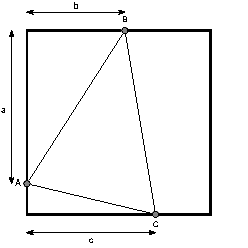
\includegraphics[width=0.7\textwidth]{triangle_sketch.pdf}
\label{definition_sketch}
\end{center}
\end{figure}

The area $A$  of the triangle can be expressed as:

\begin{eqnarray}
\label{eq_area} A &=& 1 - \frac{1}{2}(1-a) c - \frac{1}{2}a b - \frac{1}{2} ((1-c)+(1-b)) \cdot 1 \\
  &=& \frac{1}{2} (b + c - (1-a)c -ab)
\end{eqnarray}

\noindent the latter term in equation \ref{eq_area} being the area of the trapezium formed by points B and C and the righthand corners of the square.

Note that if $b$ and $c$ are equal, then the area is independent of $a$ and the largest area we can achieve then is by setting
$b$ and $c$ equal to $1$: $A = \frac{1}{2}$ (see figure \ref{triangle_area_half}).

Note also that the formula remains valid, i.e. produces a value, if the parameters $a, b, c$ become negative or larger than $1$. This is the
reason that the area has no bounds, unless we delimit the parameters to some convenient interval. It also makes it harder
to apply analytical methods to find a maximum.

\begin{figure}[h]
\begin{center}
\caption{Two triangles with area 1/2 of that of the square.}
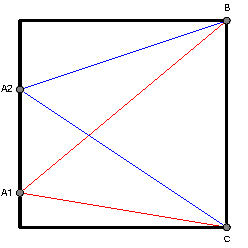
\includegraphics[width=0.7\textwidth]{triangle_area_half.pdf}
\label{triangle_area_half}
\end{center}
\end{figure}

Intuitively, this seems the largest area that a triangle within a unit square can achieve. But what about equilateral
triangles?

\subsection*{Equilateral triangles}
If the triangle is to be equilateral, we need to apply three constraints, namely the distance between
points A, B and C must be equal:

\begin{eqnarray}
  a^2 + b^2 &=& r^2 \\
  (1-a)^2 + c^2 &=& r^2 \\
\label{last_side} (c-b)^2 + 1 &=& r^2
\end{eqnarray}

We have four degrees of freedom and only three equations, so this gives us some leeway to determine the solution we like.

The equations look fairly simple, but because of the number of parameters it is difficult to solve them directly. Also,
here we have the problem that the parameters can in fact be anything and if we want a triangle that fits in the square,
then we need additional constraints, i.e. $0 \le a, b, c \le 1$.

\begin{figure}[h]
\begin{center}
\caption{The smallest equilateral triangle of which the vertices touch the side of the square.}
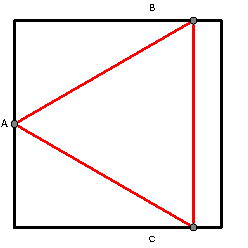
\includegraphics[width=0.7\textwidth]{triangle_smallest.pdf}
\label{triangle_smallest}
\end{center}
\end{figure}

One thing we can conclude, though, is that the side of any equilateral triangle of which the vertices lie on the sides of
the square must be at least $1$ -- see equation~\ref{last_side}. The triangle is show in figure~\ref{triangle_smallest}.
For any value of $r \ge 1$, we should be able to find
a set of parameter values that leads to an equilateral triangle, which may extend beyond the square.

Some manipulation of these equations is possible, for instance by writing the difference of $b$ and $c$ as a new parameter,
as you can then express $r$ in terms of that new parameter and eliminate $b$ or $c$. However, that does not lead to
a "nice" set of equations and it certainly does not make it easier to find "the" largest equilateral triangle.

But the possibility of constructing equilateral triangles that do not fit in the square does lead to the following
thought: by slightly tilting the equilateral triangle of figure \ref{triangle_smallest} we make the vertices come "loose"
and there is then room to enlarge it a bit. If point B hits the top-right corner we would have the largest equilateral
triangle that fits.

The parameters for this triangle can be simply found: \\
\noindent We know that $b$ will then be $1$, so that:
\begin{eqnarray}
\label{eqn_a}  a^2 + 1 &=& r^2 \\
\label{eqn_b} (1-a)^2 + c^2 &=& r^2 \\
\label{eqn_c} (1-c)^2 + 1 &=& r^2
\end{eqnarray}

From equations \ref{eqn_a} and \ref{eqn_c} we see that $a = 1 - c$, so filling this in in equation~\ref{eqn_b}:
\begin{equation}
(1-a)^2 + (1-a)^2 = a^2 + 1\\
\end{equation}

This can be rewritten as:
\begin{equation}
 a^2 - 4a + 1 = 0 \longrightarrow a = 2 - \sqrt{3}
\end{equation}
\noindent leading to the triangle in figure \ref{triangle_largest}.

Table \ref{table_triangles} summarises the properties of the triangles we found.

\begin{figure}[h]
\begin{center}
\caption{The largest equilateral triangle of which the vertices touch the side of the square.}
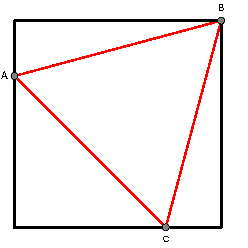
\includegraphics[width=0.7\textwidth]{triangle_largest.pdf}
\label{triangle_largest}
\end{center}
\end{figure}

\begin{table}[h]
\caption{Properties of the three triangles.}
\label{table_triangles}
\center
\begin{tabular}{llll}
\emph{Type}                   & \emph{Area}             &                    & \emph{Side} \\
Largest triangle              & $\frac{1}{2}$           & $0.500$            & $1$ and $\frac{1}{2}\sqrt{3}$ \\
Smallest equilateral triangle & $\frac{1}{4} \sqrt{3}$  & $ \approx 0.433$   & $1$ \\
Largest equilateral triangle  & $2 \sqrt{3} - 3$        & $ \approx 0.464$   & $2 \sqrt{2-\sqrt{3}} \approx 1.0353$\\
\end{tabular}
\end{table}

\emph{Note:} What is lacking is a formal proof that these triangles are indeed the largest or the smallest possible.

\end{document}
